% Apartado 2: arquitectura y comunicación entre componentes.
\section{Arquitectura y comunicación entre componentes}\label{sec:arquitectura}

El frontend está escrito en JavaScript sin framework. El backend usa FastAPI y los datos están en SQLite.
El chat va por \cod{POST /chat} y la respuesta llega en streaming con Server-Sent Events. El resto de la comunicación es
REST, es decir, peticiones HTTP normales en las que cada acción tiene su propia dirección (login, voz, banco,
operaciones, móvil simulado y ajustes) y el servidor responde con datos en JSON.

El backend sigue una arquitectura hexagonal, también llamada de puertos y adaptadores. Las dependencias solo apuntan
hacia dentro, y el dominio no sabe que existen FastAPI, SQLite, Groq ni la voz. \ruta{backend/composicion.py} es el único
fichero que conoce todas las implementaciones. \ruta{tests/test_arquitectura.py} analiza los imports y falla si una capa
interior importa una exterior. La tabla siguiente resume qué hay en cada capa y la figura~\ref{fig:arquitectura} muestra las piezas y sus
dependencias.

\begin{figure}[!htb]
  \centering
  % Diagrama de arquitectura en TikZ.
% Cajas por capa: navegador, adaptadores de entrada, aplicación, dominio, adaptadores de salida y
% proveedores de modelos. Flecha continua: llamada o dependencia. Discontinua: implementa.
% Capa fondo por debajo de background para que la caja de backend/ no tape las de cada capa.
\pgfdeclarelayer{fondo}
\pgfsetlayers{fondo,background,main}
\resizebox{0.8\textwidth}{!}{%
\begin{tikzpicture}[
    font=\sffamily\small,
    pieza/.style={draw=unicajaPetroleo, fill=white, rounded corners=2pt, align=center,
                  text width=3.4cm, minimum height=1.05cm, inner sep=3pt,
                  execute at begin node={\hyphenpenalty=10000\exhyphenpenalty=10000}},
    externo/.style={pieza, fill=unicajaAvisoClaro, draw=unicajaAviso},
    capa/.style={draw=#1, rounded corners=4pt, inner sep=7pt, line width=0.7pt},
    etiqueta/.style={font=\sffamily\footnotesize\bfseries, anchor=south west, inner sep=2pt},
    flecha/.style={-{Stealth[length=2.4mm]}, line width=0.6pt, draw=unicajaTinta},
    implementa/.style={-{Stealth[length=2.4mm]}, dashed, line width=0.6pt, draw=unicajaVerde},
    texto flecha/.style={font=\sffamily\scriptsize, fill=white, inner sep=1.5pt},
  ]

  % ---------- Navegador (frontend/js) ----------
  \node[pieza] (UI)  at (0,0)    {ui/ · tarjetas,\\ gráficos, móvil simulado};
  \node[pieza] (APP) at (4.4,0)  {aplicacion/\\conversacion.js};
  \node[pieza] (API) at (8.8,0)  {api/ · fetch + SSE};
  \node[pieza] (DIS) at (13.2,0) {dispositivos/ ·\\ micrófono, altavoz};

  % ---------- Adaptadores de entrada ----------
  \node[pieza] (R) at (8.8,-3.2) {rutas FastAPI · SSE ·\\ errores → HTTP};

  % ---------- Aplicación ----------
  \node[pieza] (CU)  at (0,-5.6)    {casos de uso: banco, bizum, tarjetas, acceso, voz, uso};
  \node[pieza] (REG) at (4.4,-5.6)  {RegistroHerramientas};
  \node[pieza] (AG)  at (8.8,-5.6)  {Agente (bucle de\\ tool calling)};
  \node[pieza] (CH)  at (13.2,-5.6) {ServicioChat};
  \node[pieza, fill=unicajaInfoClaro] (P) at (6.6,-7.5) {puertos (Protocol)};

  % ---------- Dominio y composición ----------
  \node[pieza, fill=unicajaExitoClaro, text width=3.6cm] (D) at (0,-9.9)
        {reglas · modelos · errores · uso · operaciones OTP};
  \node[pieza, fill=unicajaFondo] (COMP) at (13.2,-9.9) {composicion.py\\(cablea todo)};

  % ---------- Adaptadores de salida ----------
  \node[pieza] (SQL) at (0,-12.6)    {sqlite/ · repositorios,\\ consultor NL→SQL,\\ auditoría};
  \node[pieza] (LLM) at (4.4,-12.6)  {llm/ · cliente\\ OpenAI-compatible};
  \node[pieza] (VOZ) at (8.8,-12.6)  {voz/ · Whisper,\\ OmniVoice, Piper};
  \node[pieza] (SEG) at (13.2,-12.6) {seguridad/ · scrypt,\\ códigos, sesiones};

  % ---------- Proveedores de modelos ----------
  \node[externo] (GROQ) at (2.2,-15.4) {Groq (nube)};
  \node[externo] (OLL)  at (6.6,-15.4) {Ollama (local)};

  % ---------- Cajas de capa ----------
  \begin{scope}[on background layer]
    \node[capa=unicajaPetroleo, fill=unicajaInfoClaro!60, fit=(UI)(APP)(API)(DIS)] (NAV) {};
    \node[etiqueta, text=unicajaPetroleo] at (NAV.north west) {Navegador (frontend/js)};

    \node[capa=unicajaPetroleoOscuro, fill=unicajaBordeClaro, fit=(R)] (ENT) {};
    \node[etiqueta, text=unicajaPetroleoOscuro] at (ENT.north west) {adaptadores/entrada/http};

    \node[capa=unicajaPetroleoOscuro, fill=unicajaBordeClaro, fit=(CU)(REG)(AG)(CH)(P)] (APLI) {};
    \node[etiqueta, text=unicajaPetroleoOscuro] at (APLI.north west) {aplicacion};

    \node[capa=unicajaVerde, fill=unicajaExitoClaro!60, fit=(D)] (DOM) {};
    \node[etiqueta, text=unicajaVerde] at (DOM.north west) {dominio};

    \node[capa=unicajaPetroleoOscuro, fill=unicajaBordeClaro, fit=(SQL)(LLM)(VOZ)(SEG)] (SAL) {};
    \node[etiqueta, text=unicajaPetroleoOscuro] at (SAL.north west) {adaptadores/salida};

  \end{scope}
  \begin{pgfonlayer}{fondo}
    \node[capa=unicajaPetroleo, fill=unicajaFondo, inner sep=14pt,
          fit=(ENT)(APLI)(DOM)(SAL)(COMP)] (BACK) {};
    \node[etiqueta, text=unicajaPetroleo] at (BACK.north west) {backend/};
  \end{pgfonlayer}

  % ---------- Flechas dentro del navegador ----------
  \draw[flecha] (UI) -- (APP);
  \draw[flecha] (APP) -- (API);

  % ---------- Navegador → backend ----------
  \draw[flecha] (API) -- node[texto flecha, right=2pt, fill=none] {REST + SSE} (R);

  % ---------- Entrada → aplicación ----------
  \draw[flecha] (R.east) -| (CH.north);
  \draw[flecha] (R.west) -| (CU.north);

  % ---------- Dentro de la aplicación ----------
  \draw[flecha] (CH) -- (AG);
  \draw[flecha] (AG) -- (REG);
  \draw[flecha] (REG) -- (CU);
  \draw[flecha] (CU) -- (P);
  \draw[flecha] (AG) -- (P);

  % ---------- Casos de uso → dominio ----------
  \draw[flecha] (CU) -- (D);

  % ---------- Adaptadores de salida que implementan los puertos ----------
  \draw[implementa] (SQL) -- node[texto flecha, pos=0.35, sloped] {implementa} (P);
  \draw[implementa] (LLM) -- node[texto flecha, pos=0.35, sloped] {implementa} (P);
  \draw[implementa] (VOZ) -- node[texto flecha, pos=0.35, sloped] {implementa} (P);
  \draw[implementa] (SEG) -- node[texto flecha, pos=0.35, sloped] {implementa} (P);

  % ---------- LLM → proveedores ----------
  \draw[flecha] (LLM) -- (GROQ);
  \draw[flecha] (LLM) -- (OLL);
\end{tikzpicture}%
}

  \caption{Arquitectura hexagonal de Unia. Las flechas continuas son llamadas o dependencias. Las discontinuas son
  adaptadores que implementan un puerto.}
  \label{fig:arquitectura}
\end{figure}

{\small
\begin{tabularx}{\textwidth}{@{}P{2.9cm}P{4.6cm}L@{}}
\toprule
\textbf{Capa} & \textbf{Carpeta} & \textbf{Contiene} \\
\midrule
Dominio & \ruta{backend/dominio/} & Entidades, reglas (topes del Bizum, validación del SQL, elección de tarjeta), errores por categoría, presupuesto de tokens \\
Aplicación & \ruta{backend/aplicacion/} & Casos de uso, agente, servicio de chat, registro de herramientas, prompt y puertos \\
Adaptadores de entrada & \ruta{backend/adaptadores/entrada/http/} & Rutas FastAPI, protocolo SSE, traducción de errores a HTTP \\
Adaptadores de salida & \ruta{backend/adaptadores/salida/} & SQLite, LLM, voz, seguridad, persistencia del estado, reloj \\
\bottomrule
\end{tabularx}}

El frontend sigue la misma idea en pequeño: \ruta{js/api} (backend) → \ruta{js/aplicacion} (casos de uso) →
\ruta{js/dispositivos} (APIs del navegador) → \ruta{js/ui} (DOM). La interfaz nunca llama al backend directamente.

\FloatBarrier
\subsection{Por qué esta arquitectura y en qué influye}\label{sec:por-que-hexagonal}

Tenía dos caminos más cortos. Uno era dejarlo todo en la aplicación FastAPI con funciones sueltas, lo más rápido para un
prototipo y, de hecho, como empezó el proyecto. El otro era usar un framework de agentes, como LangChain o
un SDK de agentes, que ya trae hecho el bucle de herramientas. Ese framework me habría ahorrado escribir el bucle, pero
las guardas del apartado~\ref{sec:bucle} van dentro de él y el agente habría dependido de una biblioteca externa en
lugar de un puerto propio.

Elegí la arquitectura hexagonal sobre todo por la seguridad. El cliente entra por la sesión y llega como parámetro a
cada puerto y a cada caso de uso. Las herramientas no tienen ningún campo para elegir otro cliente, así que el modelo no
tiene por dónde pedir datos ajenos. Eso no depende del prompt.
La conocí en las prácticas extracurriculares que estoy haciendo ahora mismo, y al aplicarla en este proyecto vi de
verdad su utilidad.

También quería poder probarlo todo sin red. Como cada adaptador se puede sustituir, los tests usan un LLM falso que
sigue un guion, repositorios en memoria y una SQLite temporal. Pruebo el agente, el OTP o el aislamiento entre clientes
sin gastar cuota de Groq.

Cambiar de proveedor tampoco toca el núcleo. Llama 3.3 70B, el modelo con el que empecé,
desapareció de Groq, y pasar a gpt-oss fue cambiar el nombre del modelo en la configuración. El agente no se tocó. Con la
voz pasó algo parecido. OmniVoice entró como un adaptador nuevo, con Piper de reserva, y se cableó en
\ruta{composicion.py}. Por el mismo motivo la conversación por texto sigue funcionando sin internet con el modelo
local, que para el agente es un eslabón más de la cadena.

Además, una función nueva es un caso de uso y una herramienta, y el agente no cambia. Esa es la respuesta a la pregunta
de las 40 funciones que trato en el apartado~\ref{sec:escalabilidad}.

En el día a día esto tiene un precio. Hay más ficheros y más indirección que en un prototipo plano, y para seguir una
petición hay que pasar por la ruta, el caso de uso, el puerto y el adaptador. Todo el cableado está en
\ruta{composicion.py}. El test de \ruta{tests/test_arquitectura.py}
falla si una capa interior importa una exterior, y eso obliga a pensar dónde va cada cosa antes de escribirla.

No empecé así. Reorganicé el código en capas a principios de octubre, con el proyecto ya avanzado, cuando los módulos
del prototipo mezclaban HTTP, SQL y reglas de negocio y cada cambio tocaba media aplicación.

\subsection{Comunicación del chat}\label{sec:comunicacion}

Cada evento SSE tiene la forma \cod{data: \{"tipo": ..., "dato": ...\}}. Los tipos de evento son la manera de dar
refuerzo visual sin que el modelo escriba HTML.

{\small
\begin{tabularx}{\textwidth}{@{}P{3.2cm}L@{}}
\toprule
\textbf{Evento} & \textbf{Qué pinta el frontend} \\
\midrule
\cod{delta} & Texto en streaming, token a token \\
\cod{herramienta} & Estado efímero (``Consultando saldo…'') \\
\cod{grafico} & Gráfico Chart.js con la paleta de Unicaja \\
\cod{operacion} & Tarjeta ``Confirma tu Bizum'' o ``Desbloquear tarjeta'', con campo de código y botón de huella (nunca lleva el código) \\
\cod{tarjeta} & Tarjeta bancaria visual con la marca, los últimos 4 dígitos y el estado activa o bloqueada \\
\cod{aviso} & Nota persistente (cambio de modelo, espera por límite) \\
\cod{uso} & Medidor de tokens de la cabecera \\
\cod{fin} / \cod{error} & Texto final (dispara la voz) o error legible \\
\bottomrule
\end{tabularx}}

Las sesiones de login, las operaciones pendientes, los SMS del móvil y las conversaciones se guardan en SQLite
(\ruta{salida/persistencia/sqlite_estado.py}), de modo que sobreviven a un reinicio del servidor. El token de sesión y el
código OTP de la operación se guardan solo como huella, nunca en claro. El SMS del móvil simulado sí lleva el código
escrito, como lo llevaría un SMS de verdad.

Además, un panel de cuenta fijo muestra el saldo, el IBAN enmascarado y los últimos movimientos. La figura~\ref{fig:chat} muestra el conjunto: el panel de cuenta a la izquierda y, en el chat, un gráfico seguido de su explicación en prosa y las sugerencias de preguntas.

\begin{figure}[!htb]
  \centering
  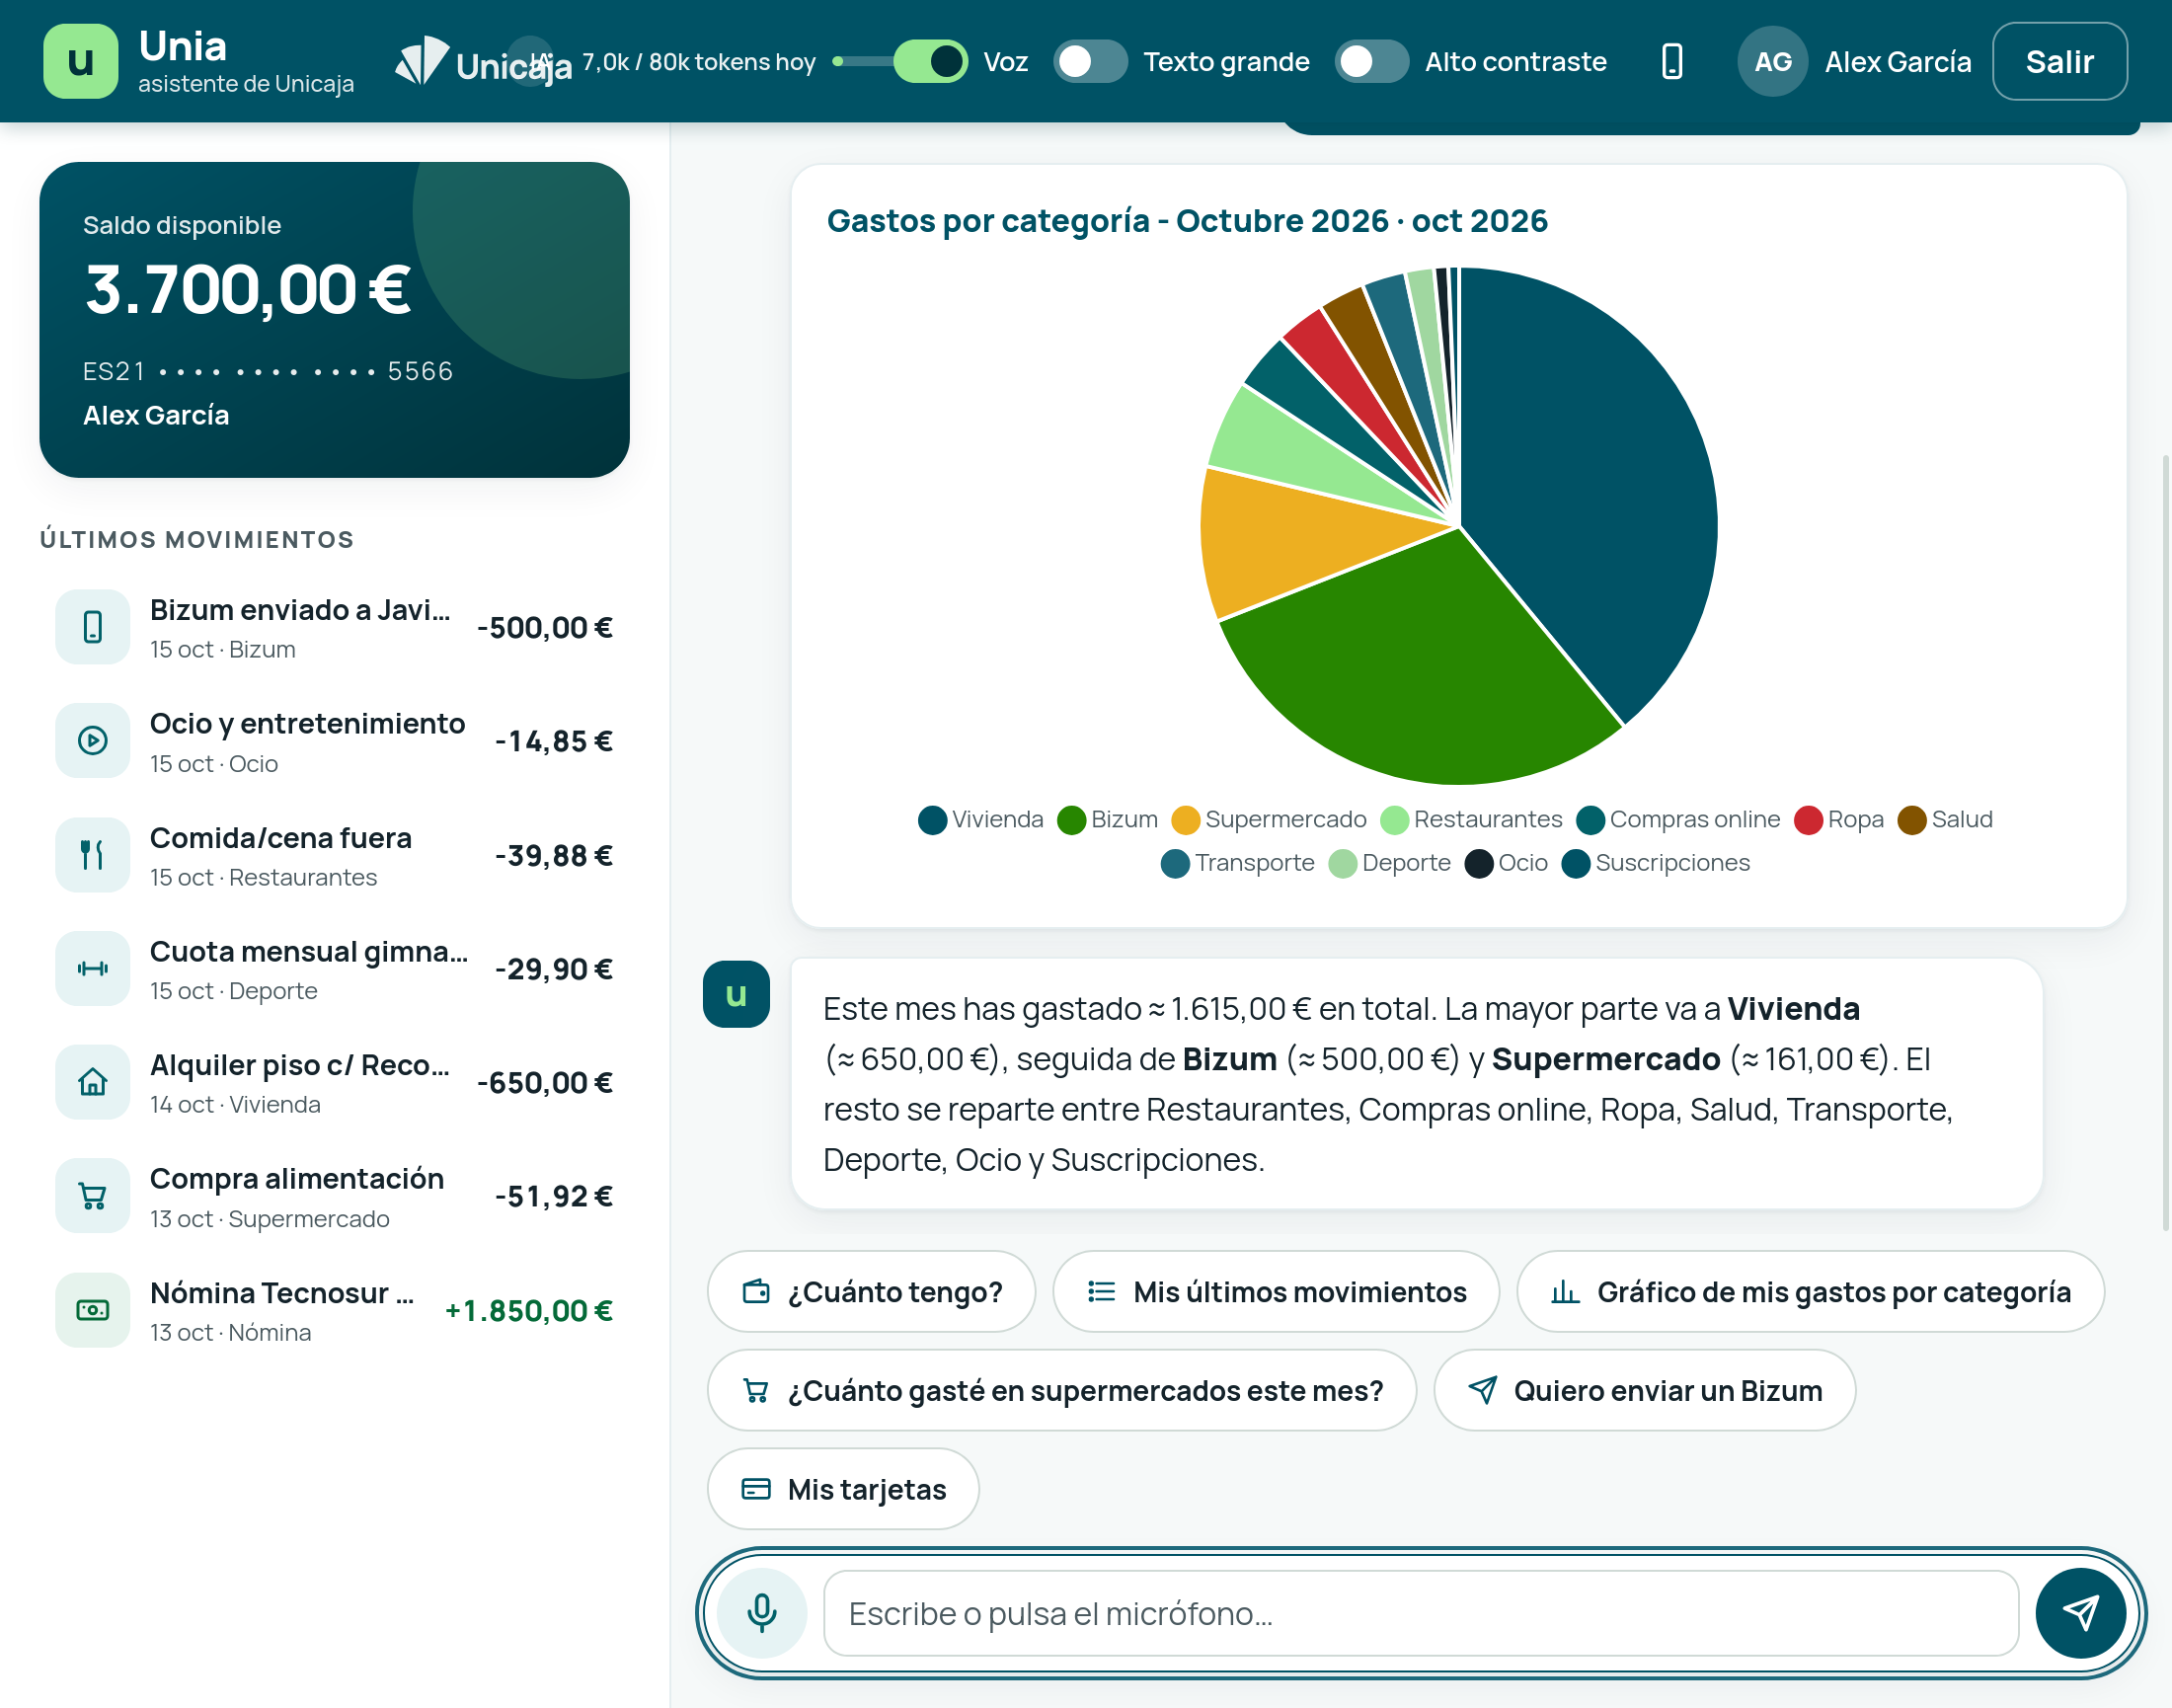
\includegraphics[width=0.95\textwidth]{figuras/chat_grafico.png}
  \caption{La interfaz tras pedir un gráfico de gastos del mes. El gráfico llega como un evento SSE propio y el modelo lo acompaña de una conclusión en prosa, que es lo que se lee en voz alta.}
  \label{fig:chat}
\end{figure}
